\documentclass{beamer}
\usetheme{Boadilla}
\usepackage{graphicx}
\usepackage{amsmath}
\usepackage{tikz}
\usepackage{media9}
\usepackage{multimedia}
\usepackage{animate}
\usetikzlibrary{shapes.geometric, arrows}
\usepackage{xcolor}
\usepackage{graphicx}
\usepackage{tcolorbox} % For colored boxes
\usepackage{graphicx} % For image manipulation
\usebackgroundtemplate{
    \includegraphics[width=\paperwidth,height=\paperheight]{background2.png} % Replace with your image path
}

\begin{document}

\begin{frame}[plain]
    \begin{center}
        % Title in a fancy font (use a font you like)
        \Huge
        \textbf{\textcolor{black}{Attention Is All You Need}}
        
        \vspace{1cm}

        % Author details without the box
        \LARGE
        \textbf{\textcolor{black}{Presented by:}} \\
        \vspace{0.4cm}
        \textbf{\textcolor{black}{Shemanty Mahjabin (2105091)}} \\ and \\ \textbf{\textcolor{black}{Mahbuba Sharmin Mim (2105103)}}

        \vspace{1cm}

    \end{center}
\end{frame}



\begin{frame}
    \frametitle{The Problem}
    \begin{columns}
        % Column 1: Text
        \begin{column}{0.6\textwidth}
            \begin{center}
                \huge \textbf{Alice’s Translation Challenge} \\
                \vspace{0.5cm}
                \large Alice is a Data Scientist. She had been tasked with building a model to  translate long, complex sentences from English to french.She was using RNNs to do it.But something was amiss. \\
               
            \end{center}
        \end{column}
        % Column 2: Alice's Image
        \begin{column}{0.4\textwidth}
            \begin{center}
                \includegraphics[width=\textwidth]{alice.png}
            \end{center}
        \end{column}
    \end{columns}
\end{frame}


% Slide 2: Problems with RNNs and CNNs
\begin{frame}
    \frametitle{RNNs \& CNNs to the Rescue... Not Quite!}
    \begin{itemize}
        \item \textbf{RNNs:}
            \begin{itemize}
                \item Slow training due to sequential processing
                \item Struggles with long-range dependencies
                \item Difficulty in capturing complex relationships in long sentences
            \end{itemize}
        \item \textbf{CNNs:}
            \begin{itemize}
                \item Limited ability to handle sequential data
                \item Cannot capture long-range dependencies effectively
                \item Struggles with understanding full context of a sentence
            \end{itemize}
    \end{itemize}
\end{frame}



% Slide 3: Enter the Transformer
\begin{frame}
    \frametitle{Enter The Transformer}
    \begin{center}
        \begin{tikzpicture}
            % Draw door and text
            \node[draw, rectangle, minimum width=5cm, minimum height=4cm] (door) at (0,0) {};
            \node at (0,0) {\includegraphics[width=5cm]{transformer.png}}; % Placeholder for door image
            
            % Text for Transformer
           
        \end{tikzpicture}
    \end{center}
    \begin{center}
       
        \large"I don’t rely on sequential processing like RNNs." \\[0.5cm]
        \pause
        \large"I use self-attention to process the entire sequence at once." \\
    \end{center}
\end{frame}

% Slide 4: Transformer’s Core Idea - Attention Mechanism
\begin{frame}
    \frametitle{Transformer’s Core Idea - Attention Mechanism}
    \begin{itemize}
        \item \textbf{Self-Attention:} Models dependencies between all words in the sequence, regardless of their position.
        \pause
        \item \textbf{Parallel Processing:} Unlike RNNs, no sequential processing—allowing faster training.
        \pause
        \item \textbf{Scalability:} Handles long-range dependencies better than RNNs and CNNs.
        \pause
        \item \textbf{Contextual Understanding:} Every word in the sequence can directly attend to every other word, improving context understanding.
    \end{itemize}
\end{frame}


\begin{frame}
    \frametitle{Transformer}
     
        \large \textbf{Goal}: To take in a piece of text and predict what word comes next.\\
    % Display the transformer image first
    
    \begin{center}
        \includegraphics[width=12cm]{je_suis_e_tudiant__2_-removebg-preview.png}
       
    \end{center}
\end{frame}

\begin{frame}{Tokens}
    
    {\textbf{Token:} Little pieces of the input text.}\\[1em]

    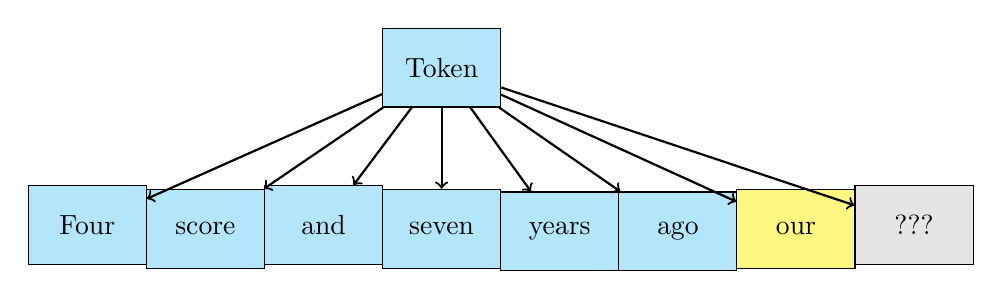
\begin{tikzpicture}[every node/.style={anchor=base,minimum width=1.5cm,minimum height=1cm,draw,align=center}]
        \node[fill=cyan!30] (token) at (4.5, 2) {Token};

        \node[fill=cyan!30] (token1) at (0, 0) {Four};
        \node[fill=cyan!30] (token2) at (1.5, 0) {score};
        \node[fill=cyan!30] (token3) at (3, 0) {and};
        \node[fill=cyan!30] (token4) at (4.5, 0) {seven};
        \node[fill=cyan!30] (token5) at (6, 0) {years};
        \node[fill=cyan!30] (token6) at (7.5, 0) {ago};
        \node[fill=yellow!50] (token7) at (9, 0) {our};
        \node[fill=gray!20] (token8) at (10.5, 0) {???};

        \draw[->,thick] (token) -- (token1);
        \draw[->,thick] (token) -- (token2);
        \draw[->,thick] (token) -- (token3);
        \draw[->,thick] (token) -- (token4);
        \draw[->,thick] (token) -- (token5);
        \draw[->,thick] (token) -- (token6);
        \draw[->,thick] (token) -- (token7);
        \draw[->,thick] (token) -- (token8);
    \end{tikzpicture}

   
    
\end{frame}



\begin{frame}{Tokens and Embeddings}

    {\textbf{Embedding: } Associating each token with a high-dimensional vector.}\\[1em]

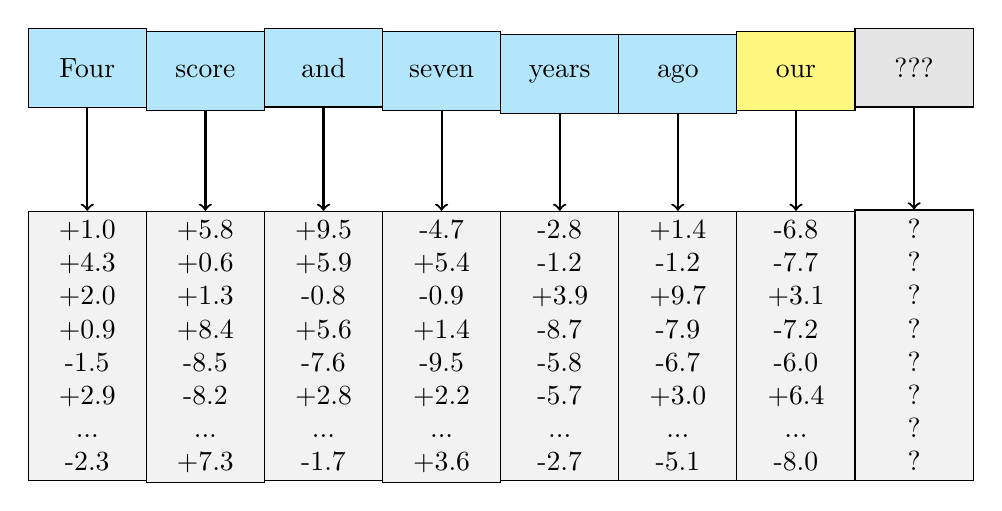
\begin{tikzpicture}[every node/.style={anchor=base,minimum width=1.5cm,minimum height=1cm,draw,align=center}]
  % Token Nodes
         % Token Nodes
  \node[fill=cyan!30] (token1) at (0, 2) {Four};
  \node[fill=cyan!30] (token2) at (1.5, 2) {score};
  \node[fill=cyan!30] (token3) at (3, 2) {and};
  \node[fill=cyan!30] (token4) at (4.5, 2) {seven};
  \node[fill=cyan!30] (token5) at (6, 2) {years};
  \node[fill=cyan!30] (token6) at (7.5, 2) {ago};
  \node[fill=yellow!50] (token7) at (9, 2) {our};
  \node[fill=gray!20] (token8) at (10.5, 2) {???};
\pause
  % Embedding Nodes
  \node[fill=gray!10,minimum height=2.5cm] (embed1) at (0, -3) {+1.0\\+4.3\\+2.0\\+0.9\\-1.5\\+2.9\\...\\-2.3};
  \node[fill=gray!10,minimum height=2.5cm] (embed2) at (1.5, -3) {+5.8\\+0.6\\+1.3\\+8.4\\-8.5\\-8.2\\...\\+7.3};
  \node[fill=gray!10,minimum height=2.5cm] (embed3) at (3, -3) {+9.5\\+5.9\\-0.8\\+5.6\\-7.6\\+2.8\\...\\-1.7};
  \node[fill=gray!10,minimum height=2.5cm] (embed4) at (4.5, -3) {-4.7\\+5.4\\-0.9\\+1.4\\-9.5\\+2.2\\...\\+3.6};
  \node[fill=gray!10,minimum height=2.5cm] (embed5) at (6, -3) {-2.8\\-1.2\\+3.9\\-8.7\\-5.8\\-5.7\\...\\-2.7};
  \node[fill=gray!10,minimum height=2.5cm] (embed6) at (7.5, -3) {+1.4\\-1.2\\+9.7\\-7.9\\-6.7\\+3.0\\...\\-5.1};
  \node[fill=gray!10,minimum height=2.5cm] (embed7) at (9, -3) {-6.8\\-7.7\\+3.1\\-7.2\\-6.0\\+6.4\\...\\-8.0};
  \node[fill=gray!10,minimum height=2.5cm] (embed8) at (10.5, -3) {?\\?\\?\\?\\?\\?\\?\\?};

  % Arrows
  \draw[->,thick] (token1) -- (embed1);
  \draw[->,thick] (token2) -- (embed2);
  \draw[->,thick] (token3) -- (embed3);
  \draw[->,thick] (token4) -- (embed4);
  \draw[->,thick] (token5) -- (embed5);
  \draw[->,thick] (token6) -- (embed6);
  \draw[->,thick] (token7) -- (embed7);
  \draw[->,thick] (token8) -- (embed8);
\end{tikzpicture}

\end{frame}



\begin{frame}{Attention in Transformers}

    

    \begin{tikzpicture}[every node/.style={anchor=base}]
        % Words on the left
        
        \draw[->,thick] (0, 5) -- (5, 5) node[midway, above] {\textbf{Embedding}};
        \node at (-1,5) {\textbf{Words}}
        \node at (7,5) {\textbf{Vectors}}
        \node at (-1, 4) {All};
        \node at (-1, 3.5) {data};
        \node at (-1, 3) {in};
        \node at (-1, 2.5) {deep};
        \node at (-1, 2) {learning};
        \node at (-1, 1.5) {must};
        \node at (-1, 1) {be};
        \node at (-1, 0.5) {represented};
        \node at (-1, 0) {as};
        \node at (-1, -0.5) {vectors};

        % Arrows to embeddings
        \draw[->,thick] (0, 4) -- ++(2,0);
        \draw[->,thick] (0, 3.5) -- ++(2,0);
        \draw[->,thick] (0, 3) -- ++(2,0);
        \draw[->,thick] (0, 2.5) -- ++(2,0);
        \draw[->,thick] (0, 2) -- ++(2,0);
        \draw[->,thick] (0, 1.5) -- ++(2,0);
        \draw[->,thick] (0, 1) -- ++(2,0);
        \draw[->,thick] (0, 0.5) -- ++(2,0);
        \draw[->,thick] (0, 0) -- ++(2,0);
        \draw[->,thick] (0, -0.5) -- ++(2,0);
\pause
        % Embedding vectors
        \node[fill=gray!20,align=center] (vector_space) at (6, 0) {
            \begin{tikzpicture}[scale=0.5]
                \draw[->] (0, 0) -- (3, 0) node[right] {x};
                \draw[->] (0, 0) -- (0, 3) node[above] {y};
                \draw[->] (0, 0) -- (1.5, 2) node[right] {in};
                \draw[->] (0, 0) -- (2, 1) node[right] {must};
                \draw[->] (0, 0) -- (-2, -1) node[left] {All};
                \draw[->] (0, 0) -- (-1, 2) node[left] {data};
                \draw[->] (0, 0) -- (1, -2) node[right] {deep};
                \draw[->] (0, 0) -- (-1.5, -2) node[left] {learning};
                \draw[->] (0, 0) -- (0.5, -1.5) node[right] {be};
                \draw[->] (0, 0) -- (-0.5, 1.5) node[left] {represented};
                \draw[->] (0, 0) -- (1, 0.5) node[right] {as};
                \draw[->] (0, 0) -- (-1, -0.5) node[left] {vectors};
            \end{tikzpicture}
        };

        % Caption
        
    \end{tikzpicture}
\end{frame}

\begin{frame}{Attention in Transformers}
    \centering

    \begin{tikzpicture}[every node/.style={anchor=base,minimum width=1.5cm,minimum height=1cm,draw,align=center}]
        
        % Word Nodes (Adjusted for proper spacing and y value of 4.5)
        \node[fill=gray!20] (word1) at (0, 4.5) {a};
        \node[fill=gray!20] (word2) at (1.5, 4.5) {fluffy};
        \node[fill=gray!20] (word3) at (3, 4.5) {blue};
        \node[fill=gray!20] (word4) at (4.5, 4.5) {creature};
        \node[fill=gray!20] (word5) at (6, 4.5) {roamed};
        \node[fill=gray!20] (word6) at (7.5, 4.5) {the};
        \node[fill=gray!20] (word7) at (9, 4.5) {verdant};
        \node[fill=gray!20] (word8) at (10.5, 4.5) {forest};
        \pause
        % Image Nodes (y = 6 for the images)
\node[fill=gray!20] (image2) at (1.5, 6) {\includegraphics[width=1.2cm, height=1.2cm]{fluffy.png}};
\node[fill=gray!20] (image3) at (3, 6) {\includegraphics[width=1.2cm, height=1.2cm]{image2.png}};
\node[fill=gray!20] (image4) at (4.5, 6) {\includegraphics[width=1.2cm, height=1.2cm]{creature1.png}};
\node[fill=gray!20] (image7) at (9, 6) {\includegraphics[width=1.2cm, height=1.2cm]{image3.png}};
\node[fill=gray!20] (image8) at (10.5, 6) {\includegraphics[width=1.2cm, height=1.2cm]{image6.png}};

        % Vector Nodes (Spacing adjusted with y value of 1.8 for vectors)
        \node[fill=gray!20] (vector1) at (0, 1.8) {\begin{tabular}{c} 6.0 \\ 0.2 \\ 3.0 \\ 6.5 \\ -  \\ - \\ 3.0 \end{tabular}};
        \node[fill=gray!20] (vector2) at (1.5, 1.8) {\begin{tabular}{c} 5.6 \\ 5.8 \\ 6.5 \\ 5.7 \\ - \\ - \\  3.6 \end{tabular}};
        \node[fill=gray!20] (vector3) at (3, 1.8) {\begin{tabular}{c} 8.8 \\ 8.0 \\ 7.0 \\ 9.1 \\ - \\ - \\ 8.6 \end{tabular}};
        \node[fill=gray!20] (vector4) at (4.5, 1.8) {\begin{tabular}{c} 1.6 \\ 6.1 \\ 1.2 \\ 8.4 \\ - \\ - \\ 6.9 \end{tabular}};
        \node[fill=gray!20] (vector5) at (6, 1.8) {\begin{tabular}{c} 4.5 \\ 7.1 \\ 9.7 \\ 8.6 \\ - \\ - \\1.7 \end{tabular}};
        \node[fill=gray!20] (vector6) at (7.5, 1.8) {\begin{tabular}{c} 5.2 \\ 0.5 \\ 2.0 \\ 0.2 \\ - \\ -  \\ 7.0 \end{tabular}};
        \node[fill=gray!20] (vector7) at (9, 1.8) {\begin{tabular}{c} 0.3 \\ 1.6 \\ 6.2 \\ 5.7 \\ - \\ - \\ 6.8 \end{tabular}};
        \node[fill=gray!20] (vector8) at (10.5, 1.8) {\begin{tabular}{c} 7.2 \\ 3.1 \\ 2.1 \\ 3.9 \\ -\\ - \\  2.3 \end{tabular}};
        
        % Arrows from Words to Images and Vectors
        
        \draw[->,thick] (word2) -- (image2);
        \draw[->,thick] (word3) -- (image3);
        \draw[->,thick] (word4) -- (image4);
        \draw[->,thick] (word7) -- (image7);
        \draw[->,thick] (word8) -- (image8);
        \draw[->,thick] (word1) -- (vector1);
        \draw[->,thick] (word2) -- (vector2);
        \draw[->,thick] (word3) -- (vector3);
        \draw[->,thick] (word4) -- (vector4);
    \end{tikzpicture}

\end{frame}


\begin{frame}{}
    \centering
    % Define the image locations
    \begin{tikzpicture}[every node/.style={anchor=mid}]

 \node (image1) at (1.5, 4) {\includegraphics[width=2cm, height=2cm]{fluffy.png}};
\node (image2) at (3.5, 4) {\includegraphics[width=2cm, height=2cm]{image2.png}};
\node (image3) at (4.5, 4) {\includegraphics[width=2cm, height=2cm]{creature1.png}};
\node (image4) at (9, 4) {\includegraphics[width=2cm, height=2cm]{image3.png}};
\node (image5) at (10.5, 4) {\includegraphics[width=2cm, height=2cm]{image6.png}};


        % Text row (middle row)
        \node (text1) at (0, 3) {\textbf{a}};
        \node (text2) at (1.5, 3) {\textbf{fluffy}};
        \node (text3) at (3, 3) {\textbf{blue}};
        \node (text4) at (4.5, 3) {\textbf{creature}};
        \node (text5) at (6, 3) {\textbf{roamed}};
        \node (text6) at (7.5, 3) {\textbf{the}};
        \node (text7) at (9, 3) {\textbf{verdant}};
        \node (text8) at (10.5, 3) {\textbf{forest}};

        % Middle row vectors
        \node (vec1) at (0, 2) {$\vec{E}_1$};
        \node (vec2) at (1.5, 2) {$\vec{E}_2$};
        \node (vec3) at (3, 2) {$\vec{E}_3$};
        \node (vec4) at (4.5, 2) {$\vec{E}_4$};
        \node (vec5) at (6, 2) {$\vec{E}_5$};
        \node (vec6) at (7.5, 2) {$\vec{E}_6$};
        \node (vec7) at (9, 2) {$\vec{E}_7$};
        \node (vec8) at (10.5, 2) {$\vec{E}_8$};

        % Bottom row vectors
        \node (vecp1) at (0, 0) {$\vec{E}'_1$};
        \node (vecp2) at (1.5, 0) {$\vec{E}'_2$};
        \node (vecp3) at (3, 0) {$\vec{E}'_3$};
        \node (vecp4) at (4.5, 0) {$\vec{E}'_4$};
        \node (vecp5) at (6, 0) {$\vec{E}'_5$};
        \node (vecp6) at (7.5, 0) {$\vec{E}'_6$};
        \node (vecp7) at (9, 0) {$\vec{E}'_7$};
        \node (vecp8) at (10.5, 0) {$\vec{E}'_8$};
\pause
        % Faint blurry lines (all connections)
        \foreach \i in {1,2,3,4,5,6,7,8} {
            \foreach \j in {1,2,3,4,5,6,7,8} {
                \draw[->, black!50] (vec\i.south) -- (vecp\j.north);
            }
        }
\pause
        % Bold arrows (specific connections)
        \draw[->, very thick, blue] (vec2.south) -- (vecp4.north);
        \draw[->, very thick, blue] (vec3.south) -- (vecp4.north);
        \draw[->, very thick, blue] (vec4.south) -- (vecp4.north);

        \draw[->, very thick, green] (vec7.south) -- (vecp8.north);
        \draw[->, very thick, green] (vec8.south) -- (vecp8.north);

        % Final images (bottom row)
        \node (final1) at (4.5, -2.5) {\includegraphics[width=2cm,height=2cm]{creature.png}};
        \node (final2) at (10.5, -2.5) {\includegraphics[width=2cm,height=2cm]{image4.png}};

    \end{tikzpicture}
\end{frame}













    

% Slide 5: High-Level Architecture
\begin{frame}
    \frametitle{High-Level Architecture}
    
   
    % Add the text and two-column layout
    \begin{columns}
        % First column with text
        \begin{column}{0.5\textwidth}
        \centering
            Transformer consists of -
            \centering
            \begin{itemize}
            
               \centering \item encoder block
               \centering \item decoder block
            \end{itemize} 
            
        \end{column}
        
        % Second column with the encoder-decoder image
        \begin{column}{0.6\textwidth}
            \includegraphics[width=\textwidth]{encoderdecoder-removebg-preview.png}
        \end{column}
    \end{columns}
\end{frame}


% Slide 6: Detailed Overview of Encoder and Decoder
\begin{frame}
    \frametitle{Encoder Components}
    A simple encoder consist of 2 parts :
    % Text for the first part (Self-Attention)
    \begin{itemize}
        \item \textbf{Self-Attention:} Relates each word to every other word in the sentence.
    \end{itemize}

    \pause

    % Text for the second part (Feed-Forward Neural Network)
    \begin{itemize}
        \item \textbf{Feed-Forward Neural Network:} The output of the self-attention mechanism is passed as input to this feed-forward network.
    \end{itemize}

\end{frame}

\begin{frame}
  \frametitle{Self-Attention in Transformers}

  \begin{itemize}
    \item \textbf{Key Steps:}
      \begin{itemize}
        \item Create 3 vectors: \textbf{Query, Key, Value}.
        \item \textbf{Dimensions:} 64-dimensional vectors.
        \item \textbf{Matrix Multiplication:} $Q = W_q \times \text{Embedding}$, $K = W_k \times \text{Embedding}$, $V = W_v \times \text{Embedding}$.
        \item \textbf{Weight Matrices:} $W_q, W_k, W_v$ of size $(512, 64)$.
      \end{itemize}
  \end{itemize}

  \vspace{1cm}

  % Add image here
  \begin{center}
    \includegraphics[width=0.6\textwidth]{QKV.png} % Replace with your image path
  \end{center}

\end{frame}


\begin{frame}
  \frametitle{Self-Attention: Step 1 - Calculate Score}

  \begin{itemize}
    \item \textbf{Score Calculation:} Measures the relationship between words.
    \item \textbf{Dot Product:} Compute the dot product of \textbf{Query} $q_1$ and \textbf{Key} $k$ for each word.
    \item \textbf{Purpose:} Determines how much each word is related to others in the sentence.
  \end{itemize}
\pause
  \vspace{.01cm}
\centering
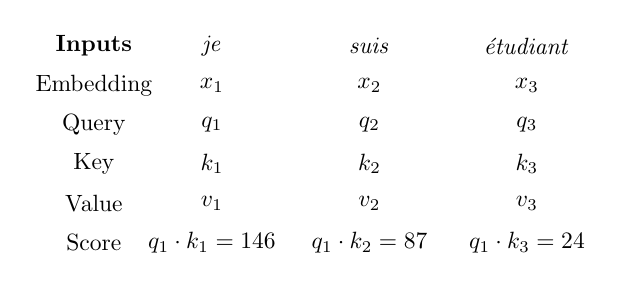
\begin{tikzpicture}[scale=1, every node/.style={scale=0.85}]
    % Nodes for inputs
    \node at (-1.5, 3.5) {\textbf{Inputs}};
    \node at (0, 3.5) {\textit{je}};
    \node at (2, 3.5) {\textit{suis}};
    \node at (4, 3.5) {\textit{étudiant}};

    % Embedding nodes
    \node at (-1.5, 3) {Embedding};
    \node at (0, 3) {$x_1$};
    \node at (2, 3) {$x_2$};
    \node at (4, 3) {$x_3$};

    % Query nodes
    \node at (-1.5, 2.5) {Query};
    \node at (0, 2.5) {$q_1$};
    \node at (2, 2.5) {$q_2$};
    \node at (4, 2.5) {$q_3$};

    % Key nodes
    \node at (-1.5, 2) {Key};
    \node at (0, 2) {$k_1$};
    \node at (2, 2) {$k_2$};
    \node at (4, 2) {$k_3$};

    % Value nodes
    \node at (-1.5, 1.5) {Value};
    \node at (0, 1.5) {$v_1$};
    \node at (2, 1.5) {$v_2$};
    \node at (4, 1.5) {$v_3$};

    % Scores
    \node at (-1.5, 1) {Score};
    \node at (0, 1) {$q_1 \cdot k_1 = 146$};
    \node at (2, 1) {$q_1 \cdot k_2 = 87$};
    \node at (4, 1) {$q_1 \cdot k_3 = 24$};
  \end{tikzpicture}

\end{frame}



\begin{frame}
  \frametitle{Self-Attention: Steps 2 & 3}

  \begin{itemize}
    \item \textbf{Step 2:} \textbf{Scale the Scores}
      \begin{itemize}
        \item Divide by $\sqrt{d_k}$ (dimension of key vectors).
        \item \textbf{Purpose:} Ensures more stable gradients.
      \end{itemize}
    \item \textbf{Step 3:} \textbf{Softmax of Scores}
      \begin{itemize}
        \item Apply softmax to scores.
        \item \textbf{Result:} Scores sum to 1.
        \item \textbf{Purpose:} Determines how much each word contributes to the output.
      \end{itemize}
  \end{itemize}

  \vspace{.01cm}

  % Add image here
\centering
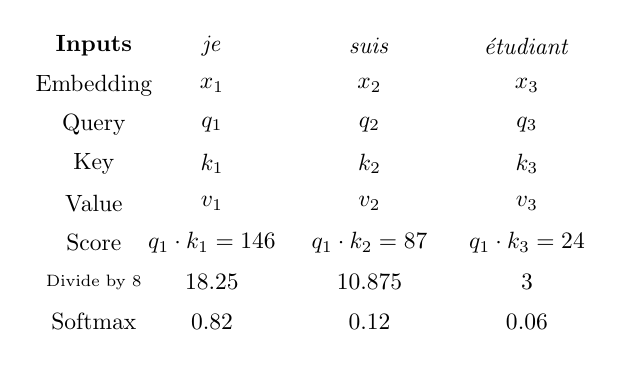
\begin{tikzpicture}[scale=1, every node/.style={scale=0.85}]
    % Nodes for inputs
    \node at (-1.5, 3.5) {\textbf{Inputs}};
    \node at (0, 3.5) {\textit{je}};
    \node at (2, 3.5) {\textit{suis}};
    \node at (4, 3.5) {\textit{étudiant}};

    % Embedding nodes
    \node at (-1.5, 3) {Embedding};
    \node at (0, 3) {$x_1$};
    \node at (2, 3) {$x_2$};
    \node at (4, 3) {$x_3$};

    % Query nodes
    \node at (-1.5, 2.5) {Query};
    \node at (0, 2.5) {$q_1$};
    \node at (2, 2.5) {$q_2$};
    \node at (4, 2.5) {$q_3$};

    % Key nodes
    \node at (-1.5, 2) {Key};
    \node at (0, 2) {$k_1$};
    \node at (2, 2) {$k_2$};
    \node at (4, 2) {$k_3$};

    % Value nodes
    \node at (-1.5, 1.5) {Value};
    \node at (0, 1.5) {$v_1$};
    \node at (2, 1.5) {$v_2$};
    \node at (4, 1.5) {$v_3$};

    % Scores
    \node at (-1.5, 1) {Score};
    \node at (0, 1) {$q_1 \cdot k_1 = 146$};
    \node at (2, 1) {$q_1 \cdot k_2 = 87$};
    \node at (4, 1) {$q_1 \cdot k_3 = 24$};
\pause
    % Divide by 8
    \node at (-1.5, 0.5) {\scriptsize Divide by 8};
    \node at (0, 0.5) {18.25};
    \node at (2, 0.5) {10.875};
    \node at (4, 0.5) {3};

    % Softmax
    \node at (-1.5, 0) {Softmax};
    \node at (0, 0) {0.82};
    \node at (2, 0) {0.12};
    \node at (4, 0) {0.06};



    % Summation
    %\node at (-1.5, -1) {\scriptsize $z_1 = \sum$};
\end{tikzpicture}

\end{frame}

\begin{frame}
  \frametitle{Self-Attention: Steps 4 & 5}

  \begin{itemize}
    \item \textbf{Step 4:} \textbf{Multiply Softmax by Value}
      \begin{itemize}
        \item Multiply softmax scores with \textbf{Value} vector $v$ for each word.
      \end{itemize}
    \item \textbf{Step 5:} \textbf{Sum to Produce Output}
      \begin{itemize}
        \item Add the results to produce a single 64-dimensional output vector.
      \end{itemize}
  \end{itemize}

  \vspace{0.6cm}

  % Add image here
\centering
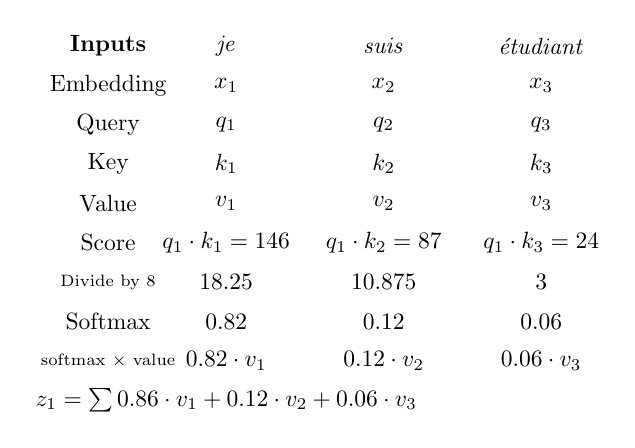
\begin{tikzpicture}[scale=1, every node/.style={scale=0.85}]
    % Nodes for inputs
    \node at (-1.5, 3.5) {\textbf{Inputs}};
    \node at (0, 3.5) {\textit{je}};
    \node at (2, 3.5) {\textit{suis}};
    \node at (4, 3.5) {\textit{étudiant}};

    % Embedding nodes
    \node at (-1.5, 3) {Embedding};
    \node at (0, 3) {$x_1$};
    \node at (2, 3) {$x_2$};
    \node at (4, 3) {$x_3$};

    % Query nodes
    \node at (-1.5, 2.5) {Query};
    \node at (0, 2.5) {$q_1$};
    \node at (2, 2.5) {$q_2$};
    \node at (4, 2.5) {$q_3$};

    % Key nodes
    \node at (-1.5, 2) {Key};
    \node at (0, 2) {$k_1$};
    \node at (2, 2) {$k_2$};
    \node at (4, 2) {$k_3$};

    % Value nodes
    \node at (-1.5, 1.5) {Value};
    \node at (0, 1.5) {$v_1$};
    \node at (2, 1.5) {$v_2$};
    \node at (4, 1.5) {$v_3$};

    % Scores
    \node at (-1.5, 1) {Score};
    \node at (0, 1) {$q_1 \cdot k_1 = 146$};
    \node at (2, 1) {$q_1 \cdot k_2 = 87$};
    \node at (4, 1) {$q_1 \cdot k_3 = 24$};

    % Divide by 8
    \node at (-1.5, 0.5) {\scriptsize Divide by 8};
    \node at (0, 0.5) {18.25};
    \node at (2, 0.5) {10.875};
    \node at (4, 0.5) {3};

    % Softmax
    \node at (-1.5, 0) {Softmax};
    \node at (0, 0) {0.82};
    \node at (2, 0) {0.12};
    \node at (4, 0) {0.06};
    \pause
    % Softmax * Value
    \node at (-1.5, -0.5) {\scriptsize softmax $\times$ value};
    \node at (0, -0.5) {$0.82 \cdot v_1$};
    \node at (2, -0.5) {$0.12 \cdot v_2$};
    \node at (4, -0.5) {$0.06 \cdot v_3$};

    % Summation
    \node at (0, -1) { $z_1 = \sum 0.86 \cdot v_1 + 0.12 \cdot v_2 + 0.06 \cdot v_3 $};
\end{tikzpicture}

  \vspace{0.01cm}


\end{frame}



\begin{frame}
  \frametitle{Multi-Head Attention}

  \begin{itemize}
    \item \textbf{Single-Head Attention:} One weight matrix (Wq, Wk, Wv) for query, key, and value.
    \item \textbf{Multi-Head Attention:} Multiple weight matrices for producing multiple queries, keys, and values.
    \item \textbf{Process:}
      \begin{itemize}
        \item Repeat the self-attention operations multiple times for each head.
        \item Combine the results from each head.
      \end{itemize}
    \item \textbf{In Transformer:} 8 Multi-Head Attention used.
  \end{itemize}
\pause
  \vspace{.01cm}

  % Add image here
  \begin{center}
    \includegraphics[width=0.6\textwidth]{multi_head_attention_image.png} % Replace with your image path
  \end{center}

\end{frame}


\begin{frame}
  \frametitle{Attention Heads and Final Output}

  \begin{itemize}
    \item \textbf{For Each Head:}
      \begin{itemize}
        \item One $Z$ matrix (attention head) per query, key, and value matrix.
      \end{itemize}
    \item \textbf{Total Heads:} 8 attention heads in the Transformer.
    \item \textbf{Final Output:} 
      \begin{itemize}
        \item Concatenate all attention heads.
        \item Multiply with other weight matrices to get the final $Z$ matrix.
      \end{itemize}
  \end{itemize}
\pause
  \vspace{.01cm}

  % Add image here
  \begin{center}
    \includegraphics[width=0.8\textwidth]{z.png} % Replace with your image path
  \end{center}

\end{frame}





\setbeamertemplate{footline}[frame number]
% Set the background image for all slides
\usebackgroundtemplate{
    \includegraphics[width=\paperwidth,height=\paperheight]{background2.png} % Replace with your image file
}

\begin{frame}
    % Slide with title in a bold and unique font style
    \frametitle{}
    \begin{center}
        % Draw a transparent rectangle around the text
        \tikz[baseline]{\node[fill=gray!20, text centered, inner sep=0.4cm, opacity=0.5] {\huge \textbf{\fontfamily{phv}\selectfont Encoder Layer - Self-Attention}};}
    \end{center}
    % After clicking, the next part of the title appears
    \frametitle{Encoder Layer - Self-Attention}
    % Add your name at the bottom of the slide
    \vfill
   
\end{frame}
\begin{frame}
    \frametitle{Encoder Input}
    \pause
    \vspace{-2cm}
    
    % Second line with arrows pointing down and variables below
    \begin{center}
        \huge
        \begin{tikzpicture}[baseline]
            % Words placed with proper spacing
            \node at (0,0) {I};
            \node at (2,0) {love};
            \node at (4.2,0) {attention};
            \node at (6.3,0) {very};
            \node at (8,0) {much};
            \pause
            % Arrows pointing down from words to x_i
            \draw[->] (0,-0.5) -- (0,-1.5);
            \draw[->] (2,-0.5) -- (2,-1.5);
            \draw[->] (4.2,-0.5) -- (4.2,-1.5);
            \draw[->] (6.3,-0.5) -- (6.3,-1.5);
            \draw[->] (8,-0.5) -- (8,-1.5);
            \pause
            % Variables below each arrow (x_1, x_2, ...)
            \node at (-1,-2) {$X$=};
            \node at (0,-2) { [ $x_1$};
            \node at (2,-2) { $x_2$};
            \node at (4.2,-2) {$x_3$};
            \node at (6.3,-2) {$x_4$};
            \node at (8,-2) {$x_5$ ]};
            
            % Arrows pointing down to x_i' with italicized and smaller PEi labels
            \draw[->] (0,-2.5) -- (0,-3.5) node[midway, right] {\scriptsize \textit{+PE$_1$}};
            \draw[->] (2,-2.5) -- (2,-3.5) node[midway, right] {\scriptsize \textit{+PE$_2$}};
            \draw[->] (4.2,-2.5) -- (4.2,-3.5) node[midway, right] {\scriptsize \textit{+PE$_3$}};
            \draw[->] (6.3,-2.5) -- (6.3,-3.5) node[midway, right] {\scriptsize \textit{+PE$_4$}};
            \draw[->] (8,-2.5) -- (8,-3.5) node[midway, right] {\scriptsize \textit{+PE$_5$}};

            % Variables x_i' below each arrow
             \node at (-1,-4) {$X'$= };
            \node at (0,-4) {[ $x_1'$};
            \node at (2,-4) {$x_2'$};
            \node at (4.2,-4) {$x_3'$};
            \node at (6.3,-4) {$x_4'$};
            \node at (8,-4) {$x_5'$ ]};
        \end{tikzpicture}
    \end{center}
\end{frame}
\begin{frame}
    \frametitle{Encoder Output}
    
    % "X'" in huge font above the matrix
    \vspace{-4cm}
    \begin{center}
        \huge $X'$
    \end{center}
    
    % Matrix with some variables and smaller size
    \[
    \begin{bmatrix}
        x_{11}' & x_{12}' & \cdots & \cdots \\
        x_{21}' & x_{22}' & \cdots & \cdots \\
        \vdots & \vdots & \vdots & \vdots \\
    \end{bmatrix}
    \]
    \pause % Pause after showing the matrix
    
    % TikZ drawing for arrows and labels with fade effect
    \begin{tikzpicture}[overlay, remember picture]
        \onslide<2->{
            \transfade
            \draw[-] (5.4,0) -- (5.4,-1);  % Central downward arrow
            \draw[->] (5.4,-1) -- (1.4,-1) -- (1.4,-2);  % Left arrow (move left then down)
            \draw[->] (5.4,-1) -- (5.4,-2);  % Straight down arrow (no label for it)
            \draw[->] (5.4,-1) -- (9.4,-1) -- (9.4,-2);  % Right arrow (move right then down)
        }
        
        \onslide<3->{
            \transfade
            % Positioning the new matrix for Q below the left arrow
            \node at (1.4,-2.5) {\huge $Q$};  % Place Q label below the left arrow
            % Matrix for Q (scaled down horizontally)
            \node at (1.4,-4) {
                \[
                \begin{bmatrix}
                    Q_{11} & Q_{12} & \cdots \\
                    Q_{21} & Q_{22} & \cdots \\
                    \vdots & \vdots & \vdots \\
                \end{bmatrix}
                \]};
        }
        
        \onslide<4->{
            \transfade
            % Positioning the new matrix for K below the straight down arrow
            \node at (5.4,-2.5) {\huge $K$};  % Place K label below the straight down arrow
            % Matrix for K (scaled down horizontally)
            \node at (5.4,-4) {
                \[
                \begin{bmatrix}
                    K_{11} & K_{12} & \cdots \\
                    K_{21} & K_{22} & \cdots \\
                    \vdots & \vdots & \vdots \\
                \end{bmatrix}
                \]};
        }
        
        \onslide<5->{
            \transfade
            % Positioning the new matrix for V below the right arrow
            \node at (9.4,-2.5) {\huge $V$};  % Place V label below the right arrow
            % Matrix for V (scaled down horizontally)
            \node at (9.4,-4) {
                \[
                \begin{bmatrix}
                    V_{11} & V_{12} & \cdots \\
                    V_{21} & V_{22} & \cdots \\
                    \vdots & \vdots & \vdots \\
                \end{bmatrix}
                \]};
        }
    \end{tikzpicture}
    
    \pause % Pause after drawing matrices
    
    % Place the dimension label directly below the matrix
    \vspace{-0.5cm}  % Adjust vertical space to position dimension correctly
    \hspace{7.5cm} % Adjust horizontal space to align dimension label with matrix
    \scriptsize \textit{($seq$, 512)}
    
    \vspace{0.5cm}
    \hspace{-7.5cm}
\end{frame}

\begin{frame}
    \frametitle{Q, K, and V}
    
    % Define complementary colors
    \definecolor{ash}{rgb}{0.6, 0.6, 0.6}  % Ash gray color
    \definecolor{softblue}{rgb}{0.4, 0.6, 0.8}  % Soft blue
    \definecolor{softgreen}{rgb}{0.4, 0.8, 0.4}  % Soft green
    \definecolor{softred}{rgb}{0.8, 0.4, 0.4}  % Soft red
    \definecolor{softpurple}{rgb}{0.6, 0.5, 0.8}  % Soft purple
    \definecolor{softyellow}{rgb}{0.9, 0.8, 0.4}  % Soft yellow (for Add & Norm)

    \begin{tikzpicture}[node distance=2cm]

    % Create rectangular nodes for Q, K, and V
    \onslide<1->{ % Q appears on slide 1
        \node[draw, fill=softblue, text=white, minimum width=2.5cm, minimum height=1.5cm, align=center] (Q) at (0, 0) {\huge \textbf{Q}};
    }
    \onslide<2->{ % K appears on slide 2
        \node[draw, fill=softgreen, text=white, minimum width=2.5cm, minimum height=1.5cm, align=center] (K) at (4, 0) {\huge \textbf{K}};
    }
    \onslide<3->{ % V appears on slide 3
        \node[draw, fill=softred, text=white, minimum width=2.5cm, minimum height=1.5cm, align=center] (V) at (8, 0) {\huge \textbf{V}};
    }
    
    % Draw arrows from the center of each rectangular node, pointing down
    \onslide<4->{ % Arrows appear on slide 4
        \draw[->, thick, color=softblue] (Q) -- (0, -2);  % Blue arrow from Q
        \draw[->, thick, color=softgreen] (K) -- (4, -2);  % Green arrow from K
        \draw[->, thick, color=softred] (V) -- (8, -2);  % Red arrow from V
    }

    % Draw the big rectangle labeled "Multihead Attention" with soft purple
    \onslide<5->{ % MHA box appears on slide 5
        \node[draw, fill=softpurple, text=white, minimum width=12cm, minimum height=2cm, align=center] (MHA) at (4, -3) {\huge \textbf{Multihead Attention}};
    }
    
    % Draw the smaller rectangle for "Add & Norm" with soft yellow
    \onslide<6->{ % Add & Norm box appears on slide 6
        \node[draw, fill=softyellow, text=white, minimum width=8cm, minimum height=1.5cm, align=center] (AddNorm) at (4, -6) {\huge \textbf{Add & Norm}};
    }
    
    % Draw the arrow from "Multihead Attention" to "Add & Norm"
    \onslide<7->{ % Arrow from Multihead to Add & Norm
        \draw[->, thick, color=softpurple] (MHA) -- (AddNorm);
    }
    
    \end{tikzpicture}
    
\end{frame}

\begin{frame}
    % Slide with title in a bold and unique font style
    \frametitle{}
    \begin{center}
        % Draw a transparent rectangle around the text with smaller text and reduced padding
        \tikz[baseline]{\node[fill=gray!20, text centered, inner sep=0.2cm, opacity=0.5] {\LARGE \textbf{\fontfamily{phv}\selectfont Encoder Layer - Feed Forward Network}};}
    \end{center}
    
    % After clicking, the next part of the title appears
    \frametitle{Encoder Layer - Feed Forward Network}
    % Add your name at the bottom of the slide
    \vfill
\end{frame}
\begin{frame}
    \frametitle{Feed Forward Processing}
    
    % First sentence of the slide
    \pause
    
    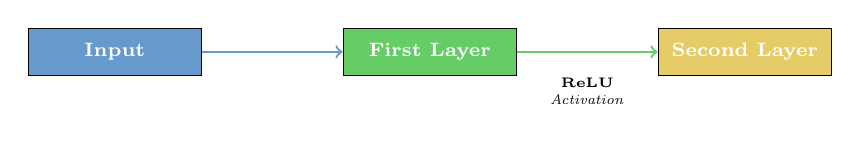
\begin{tikzpicture}[node distance=1cm]
     % Define colors for text and boxes
        
   % Define colors that complement grey
        \definecolor{softblue}{rgb}{0.4, 0.6, 0.8}  % Soft blue color
        \definecolor{softgreen}{rgb}{0.4, 0.8, 0.4}  % Soft green color
        \definecolor{softyellow}{rgb}{0.9, 0.8, 0.4}  % Soft yellow color for the circle
        
        % Draw the input box with a soft blue background (smaller box)
        \node[draw, fill=softblue, text=white, minimum width=2.2cm, minimum height=0.6cm, align=center, font=\scriptsize] (input) at (0,-1) {\textbf{Input}};
        
        % Draw the "First Layer" box with a soft green background (smaller box)
        \node[draw, fill=softgreen, text=white, minimum width=2.2cm, minimum height=0.6cm, align=center, font=\scriptsize] (firstlayer) at (4,-1) {\textbf{First Layer}};
        
        % Draw a horizontal arrow from "Input" to "First Layer"
        \draw[->, thick, color=softblue] (input) -- (firstlayer);
        
        % Add a 2D array (circle) near the "First Layer" to describe it (small circle)
        
        % Draw the "Second Layer" box with a soft yellow background (smaller box)
        \node[draw, fill=softyellow, text=white, minimum width=2.2cm, minimum height=0.6cm, align=center, font=\scriptsize] (secondlayer) at (8,-1) {\textbf{Second Layer}};
        
        % Draw a horizontal arrow from "First Layer" to "Second Layer"
        \draw[->, thick, color=softgreen] (firstlayer) -- (secondlayer);
        
        % Add "ReLU Activation" label along the arrow
        \node[align=center, font=\tiny] at (6,-1.5) {\textbf{ReLU} \\ \textit{Activation}};
        
    \end{tikzpicture}
    
\end{frame}
\begin{frame}
    \frametitle{Mathematical Formulation for Feedforward Network}
    
    \begin{itemize}
        \item \textbf{Given the output from the attention mechanism \( Z \) (for each token):}
        \pause
        \item \textbf{First Linear Transformation:}
        \[
        A_1 = \text{ReLU}(Z W_1 + b_1)
        \]
        \pause
        
        \item \textbf{Second Linear Transformation:}
        \[
        A_2 = A_1 W_2 + b_2
        \]
        \pause

        \item \textbf{Add Residual Connection:}
        \[
        Z_{\text{out}} = A_2 + Z
        \]
        \pause
        \item \textbf{Layer Normalization:}
        \[
        \text{Norm}(Z_{\text{out}})
        \]
    \end{itemize}
    
\end{frame}
\begin{frame}
    \frametitle{The Transformer}
    
    \begin{center}
        \includegraphics[width=0.6\textwidth]{t-Photoroom.png}  % Replace with your image filename
    \end{center}
    
\end{frame}

\begin{frame}
    \frametitle{Masked Multi-Head Attention}
    
    \begin{center}
        \textbf{Visualizing Masked Multihead Attention}
    \end{center}

    % Animate the images automatically, looping without controls or stopping
    \centering
    \animategraphics[autoplay,loop,scale=0.8,width=0.8\textwidth]{1}{frame}{1}{10}  % 10 is the frame rate, 1-8 are the image numbers
\end{frame}

\begin{frame}

    \frametitle{Total Flow}
   \vspace{-2}
    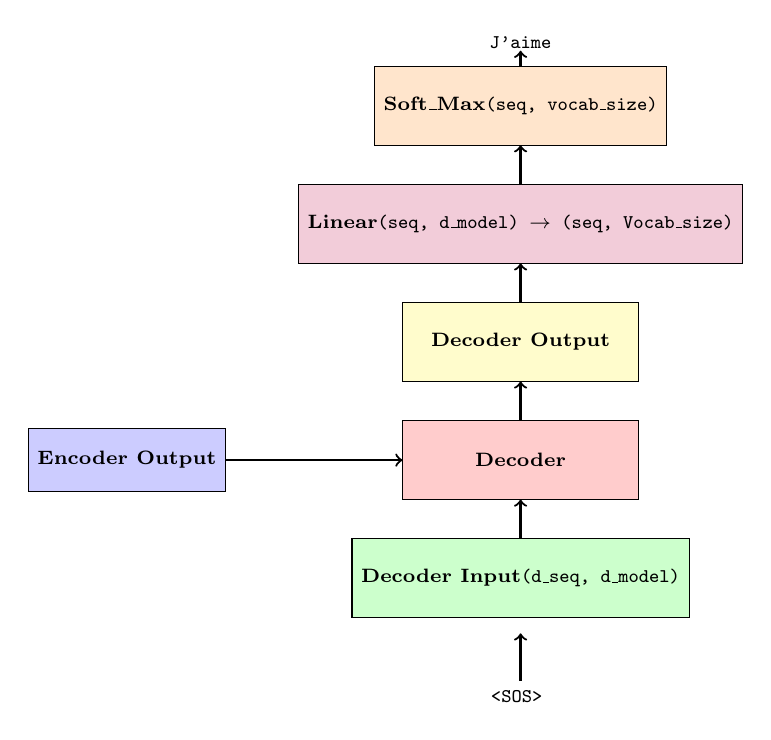
\begin{tikzpicture}
        % Draw the small rectangle for Encoder Output
        \node[draw, fill=blue!20, text centered, minimum width=2.5cm, minimum height=0.8cm] (encoder) at (0, 0) {\scriptsize \textbf{Encoder Output}};
        
        % Place the <SOS> text at the rightmost bottom of Encoder Output
        \node[anchor=west] at (4.5, -3) {\scriptsize \texttt{<SOS>}};

        % Draw an arrow from <SOS> to Decoder Input, pointing upwards
        \draw[->, thick] (5, -2.8) -- (5, -2.2);  % Arrow from <SOS> to Decoder Input
        
        % Draw the small rectangle for Decoder Input with two lines of text
        \node[draw, fill=green!20, text centered, minimum width=3cm, minimum height=1cm] (decoderInput) at (5, -1.5) {\scriptsize \textbf{Decoder Input} \\ \scriptsize \texttt{(d\_seq, d\_model)}};
        
        % Draw an arrow from Decoder Input to Decoder (pointing towards Decoder)
        \draw[->, thick] (5, -1) -- (5, -0.5);  % Arrow from Decoder Input to Decoder
        
        % Draw the small rectangle for Decoder (new rectangle)
        \node[draw, fill=red!20, text centered, minimum width=3cm, minimum height=1cm] (decoder) at (5, 0) {\scriptsize \textbf{Decoder}};
        
        % Draw an arrow from Encoder Output to Decoder (pointing towards Decoder)
        \draw[->, thick] (1.25, 0) -- (3.5, 0);  % Arrow from Encoder Output to Decoder
        \pause
        % Draw the small rectangle for Decoder Output
        \node[draw, fill=yellow!20, text centered, minimum width=3cm, minimum height=1cm] (decoderOutput) at (5, 1.5) {\scriptsize \textbf{Decoder Output}};
        
        % Draw an arrow from Decoder to Decoder Output
        \draw[->, thick] (5, 0.5) -- (5, 1);  % Arrow from Decoder to Decoder Output
       \pause
        % Draw the small rectangle for Linear with two lines of text
        \node[draw, fill=purple!20, text centered, minimum width=3cm, minimum height=1cm] (linear) at (5, 3) {\scriptsize \textbf{Linear} \\ \scriptsize \texttt{(seq, d\_model) $\rightarrow$ (seq, Vocab\_size)}};
        
        % Draw an arrow from Decoder Output to Linear
        \draw[->, thick] (5, 2) -- (5, 2.5);  % Arrow from Decoder Output to Linear
        \pause
        % Draw the small rectangle for Soft_Max with two lines of text
        \node[draw, fill=orange!20, text centered, minimum width=3cm, minimum height=1cm] (softmax) at (5, 4.5) {\scriptsize \textbf{Soft\_Max} \\ \scriptsize \texttt{(seq, vocab\_size)}};
        
        % Draw an arrow from Linear to Soft_Max
        \draw[->, thick] (5, 3.5) -- (5, 4);  % Arrow from Linear to Soft_Max
        \pause
        % Draw the text node for "je" (French for "I")
        \node at (5,5.3) {\scriptsize \texttt{J'aime}};
        
        % Draw an arrow from Soft_Max to the "je" text
        \draw[->, thick] (5, 5) -- (5, 5.2);  % Arrow from Soft_Max to "je" text
        
    \end{tikzpicture}

\end{frame}

\begin{frame}

    \frametitle{Total Flow}
   \vspace{-2}
    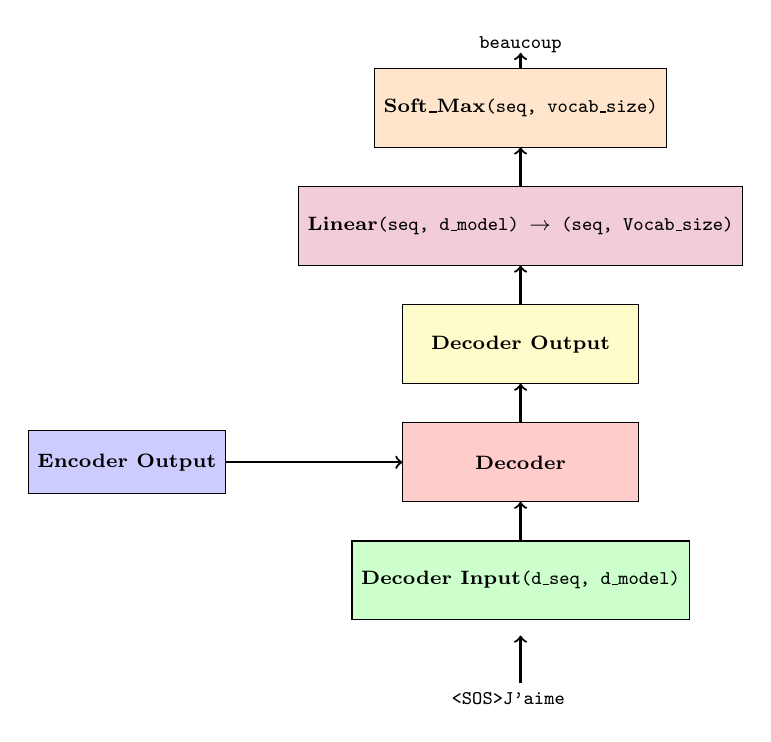
\begin{tikzpicture}
        % Draw the small rectangle for Encoder Output
        \node[draw, fill=blue!20, text centered, minimum width=2.5cm, minimum height=0.8cm] (encoder) at (0, 0) {\scriptsize \textbf{Encoder Output}};
        
        % Place the <SOS> text at the rightmost bottom of Encoder Output
        \node[anchor=west] at (4, -3) {\scriptsize \texttt{<SOS>J'aime}};

        % Draw an arrow from <SOS> to Decoder Input, pointing upwards
        \draw[->, thick] (5, -2.8) -- (5, -2.2);  % Arrow from <SOS> to Decoder Input
        
        % Draw the small rectangle for Decoder Input with two lines of text
        \node[draw, fill=green!20, text centered, minimum width=3cm, minimum height=1cm] (decoderInput) at (5, -1.5) {\scriptsize \textbf{Decoder Input} \\ \scriptsize \texttt{(d\_seq, d\_model)}};
        
        % Draw an arrow from Decoder Input to Decoder (pointing towards Decoder)
        \draw[->, thick] (5, -1) -- (5, -0.5);  % Arrow from Decoder Input to Decoder
        
        % Draw the small rectangle for Decoder (new rectangle)
        \node[draw, fill=red!20, text centered, minimum width=3cm, minimum height=1cm] (decoder) at (5, 0) {\scriptsize \textbf{Decoder}};
        
        % Draw an arrow from Encoder Output to Decoder (pointing towards Decoder)
        \draw[->, thick] (1.25, 0) -- (3.5, 0);  % Arrow from Encoder Output to Decoder
        \pause
        % Draw the small rectangle for Decoder Output
        \node[draw, fill=yellow!20, text centered, minimum width=3cm, minimum height=1cm] (decoderOutput) at (5, 1.5) {\scriptsize \textbf{Decoder Output}};
        
        % Draw an arrow from Decoder to Decoder Output
        \draw[->, thick] (5, 0.5) -- (5, 1);  % Arrow from Decoder to Decoder Output
       \pause
        % Draw the small rectangle for Linear with two lines of text
        \node[draw, fill=purple!20, text centered, minimum width=3cm, minimum height=1cm] (linear) at (5, 3) {\scriptsize \textbf{Linear} \\ \scriptsize \texttt{(seq, d\_model) $\rightarrow$ (seq, Vocab\_size)}};
        
        % Draw an arrow from Decoder Output to Linear
        \draw[->, thick] (5, 2) -- (5, 2.5);  % Arrow from Decoder Output to Linear
        \pause
        % Draw the small rectangle for Soft_Max with two lines of text
        \node[draw, fill=orange!20, text centered, minimum width=3cm, minimum height=1cm] (softmax) at (5, 4.5) {\scriptsize \textbf{Soft\_Max} \\ \scriptsize \texttt{(seq, vocab\_size)}};
        
        % Draw an arrow from Linear to Soft_Max
        \draw[->, thick] (5, 3.5) -- (5, 4);  % Arrow from Linear to Soft_Max
        \pause
        % Draw the text node for "je" (French for "I")
        \node at (5,5.3) {\scriptsize \texttt{beaucoup}};
        
        % Draw an arrow from Soft_Max to the "je" text
        \draw[->, thick] (5, 5) -- (5, 5.2);  % Arrow from Soft_Max to "je" text
        
    \end{tikzpicture}

\end{frame}
\begin{frame}

    \frametitle{Total Flow}
   \vspace{-2}
    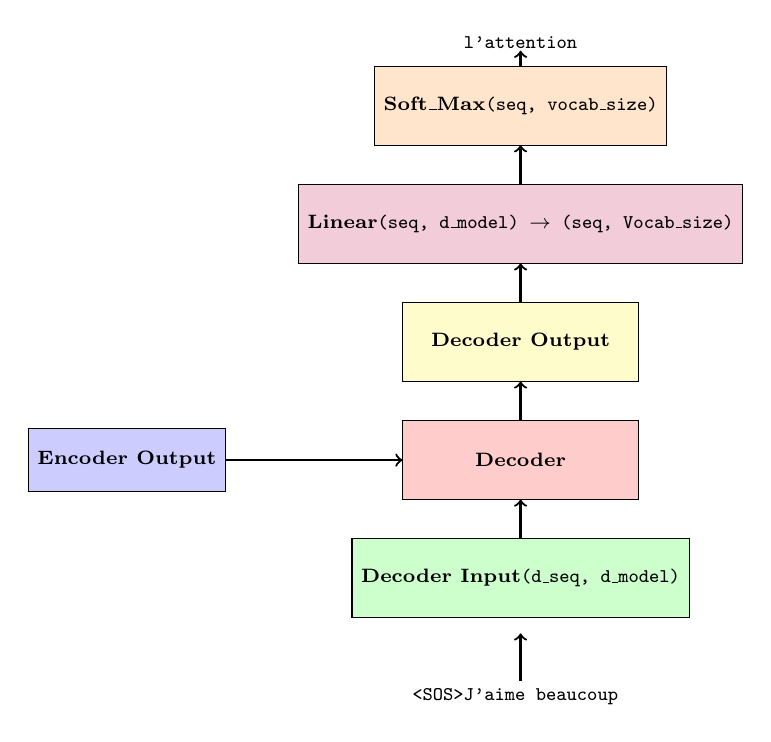
\begin{tikzpicture}
        % Draw the small rectangle for Encoder Output
        \node[draw, fill=blue!20, text centered, minimum width=2.5cm, minimum height=0.8cm] (encoder) at (0, 0) {\scriptsize \textbf{Encoder Output}};
        
        % Place the <SOS> text at the rightmost bottom of Encoder Output
        \node[anchor=west] at (3.5, -3) {\scriptsize \texttt{<SOS>J'aime beaucoup}};

        % Draw an arrow from <SOS> to Decoder Input, pointing upwards
        \draw[->, thick] (5, -2.8) -- (5, -2.2);  % Arrow from <SOS> to Decoder Input
        
        % Draw the small rectangle for Decoder Input with two lines of text
        \node[draw, fill=green!20, text centered, minimum width=3cm, minimum height=1cm] (decoderInput) at (5, -1.5) {\scriptsize \textbf{Decoder Input} \\ \scriptsize \texttt{(d\_seq, d\_model)}};
        
        % Draw an arrow from Decoder Input to Decoder (pointing towards Decoder)
        \draw[->, thick] (5, -1) -- (5, -0.5);  % Arrow from Decoder Input to Decoder
        
        % Draw the small rectangle for Decoder (new rectangle)
        \node[draw, fill=red!20, text centered, minimum width=3cm, minimum height=1cm] (decoder) at (5, 0) {\scriptsize \textbf{Decoder}};
        
        % Draw an arrow from Encoder Output to Decoder (pointing towards Decoder)
        \draw[->, thick] (1.25, 0) -- (3.5, 0);  % Arrow from Encoder Output to Decoder
        \pause
        % Draw the small rectangle for Decoder Output
        \node[draw, fill=yellow!20, text centered, minimum width=3cm, minimum height=1cm] (decoderOutput) at (5, 1.5) {\scriptsize \textbf{Decoder Output}};
        
        % Draw an arrow from Decoder to Decoder Output
        \draw[->, thick] (5, 0.5) -- (5, 1);  % Arrow from Decoder to Decoder Output
       \pause
        % Draw the small rectangle for Linear with two lines of text
        \node[draw, fill=purple!20, text centered, minimum width=3cm, minimum height=1cm] (linear) at (5, 3) {\scriptsize \textbf{Linear} \\ \scriptsize \texttt{(seq, d\_model) $\rightarrow$ (seq, Vocab\_size)}};
        
        % Draw an arrow from Decoder Output to Linear
        \draw[->, thick] (5, 2) -- (5, 2.5);  % Arrow from Decoder Output to Linear
        \pause
        % Draw the small rectangle for Soft_Max with two lines of text
        \node[draw, fill=orange!20, text centered, minimum width=3cm, minimum height=1cm] (softmax) at (5, 4.5) {\scriptsize \textbf{Soft\_Max} \\ \scriptsize \texttt{(seq, vocab\_size)}};
        
        % Draw an arrow from Linear to Soft_Max
        \draw[->, thick] (5, 3.5) -- (5, 4);  % Arrow from Linear to Soft_Max
        \pause
        % Draw the text node for "je" (French for "I")
        \node at (5,5.3) {\scriptsize \texttt{l'attention}};
        
        % Draw an arrow from Soft_Max to the "je" text
        \draw[->, thick] (5, 5) -- (5, 5.2);  % Arrow from Soft_Max to "je" text
        
    \end{tikzpicture}

\end{frame}
\begin{frame}

    \frametitle{Total Flow}
   \vspace{-2}
    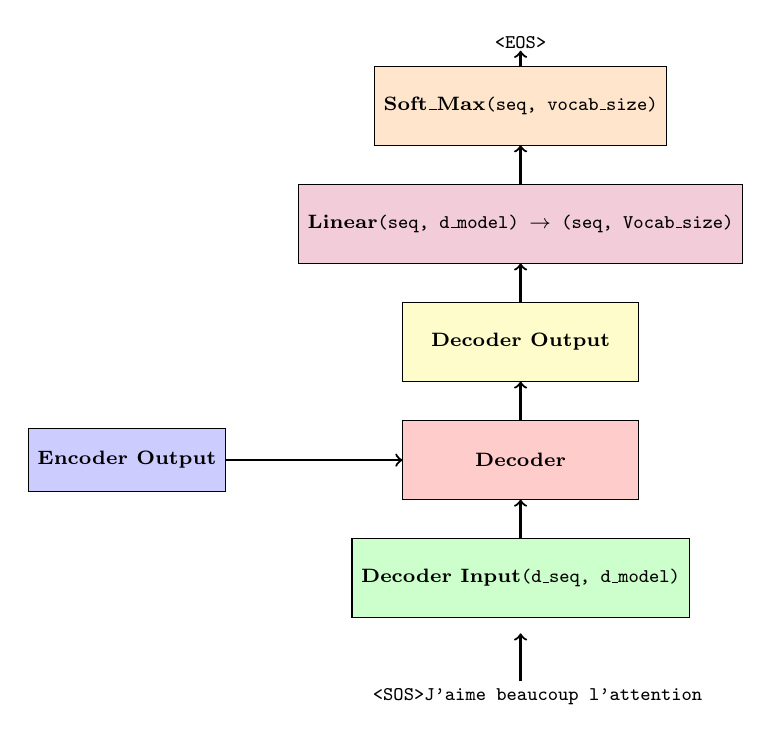
\begin{tikzpicture}
        % Draw the small rectangle for Encoder Output
        \node[draw, fill=blue!20, text centered, minimum width=2.5cm, minimum height=0.8cm] (encoder) at (0, 0) {\scriptsize \textbf{Encoder Output}};
        
        % Place the <SOS> text at the rightmost bottom of Encoder Output
        \node[anchor=west] at (3, -3) {\scriptsize \texttt{<SOS>J'aime beaucoup l'attention}};

        % Draw an arrow from <SOS> to Decoder Input, pointing upwards
        \draw[->, thick] (5, -2.8) -- (5, -2.2);  % Arrow from <SOS> to Decoder Input
        
        % Draw the small rectangle for Decoder Input with two lines of text
        \node[draw, fill=green!20, text centered, minimum width=3cm, minimum height=1cm] (decoderInput) at (5, -1.5) {\scriptsize \textbf{Decoder Input} \\ \scriptsize \texttt{(d\_seq, d\_model)}};
        
        % Draw an arrow from Decoder Input to Decoder (pointing towards Decoder)
        \draw[->, thick] (5, -1) -- (5, -0.5);  % Arrow from Decoder Input to Decoder
        
        % Draw the small rectangle for Decoder (new rectangle)
        \node[draw, fill=red!20, text centered, minimum width=3cm, minimum height=1cm] (decoder) at (5, 0) {\scriptsize \textbf{Decoder}};
        
        % Draw an arrow from Encoder Output to Decoder (pointing towards Decoder)
        \draw[->, thick] (1.25, 0) -- (3.5, 0);  % Arrow from Encoder Output to Decoder
        \pause
        % Draw the small rectangle for Decoder Output
        \node[draw, fill=yellow!20, text centered, minimum width=3cm, minimum height=1cm] (decoderOutput) at (5, 1.5) {\scriptsize \textbf{Decoder Output}};
        
        % Draw an arrow from Decoder to Decoder Output
        \draw[->, thick] (5, 0.5) -- (5, 1);  % Arrow from Decoder to Decoder Output
       \pause
        % Draw the small rectangle for Linear with two lines of text
        \node[draw, fill=purple!20, text centered, minimum width=3cm, minimum height=1cm] (linear) at (5, 3) {\scriptsize \textbf{Linear} \\ \scriptsize \texttt{(seq, d\_model) $\rightarrow$ (seq, Vocab\_size)}};
        
        % Draw an arrow from Decoder Output to Linear
        \draw[->, thick] (5, 2) -- (5, 2.5);  % Arrow from Decoder Output to Linear
        \pause
        % Draw the small rectangle for Soft_Max with two lines of text
        \node[draw, fill=orange!20, text centered, minimum width=3cm, minimum height=1cm] (softmax) at (5, 4.5) {\scriptsize \textbf{Soft\_Max} \\ \scriptsize \texttt{(seq, vocab\_size)}};
        
        % Draw an arrow from Linear to Soft_Max
        \draw[->, thick] (5, 3.5) -- (5, 4);  % Arrow from Linear to Soft_Max
        \pause
        % Draw the text node for "je" (French for "I")
        \node at (5,5.3) {\scriptsize \texttt{<EOS>}};
        
        % Draw an arrow from Soft_Max to the "je" text
        \draw[->, thick] (5, 5) -- (5, 5.2);  % Arrow from Soft_Max to "je" text
        
    \end{tikzpicture}

\end{frame}
\begin{frame}
    \frametitle{Machine Translation Results (6.1)}

    \begin{itemize}
        \item Transformer (big) outperforms all prior models on English-to-German with a BLEU score of \textbf{28.4}. \pause
        \item On English-to-French, Transformer achieves \textbf{41.0} BLEU, with \textbf{1/4 the training cost}. \pause
        \item Base models averaged the last 5 checkpoints, and beam search was used with beam size = 4. \pause
        \item Training cost is compared with other architectures, and estimated using TFLOPS. \pause
    \end{itemize}
\end{frame}
\begin{frame}
    \frametitle{Model Variations (6.2)}

    \begin{itemize}
        \item \textbf{Experiment with Transformer Components:} Varying configurations and measuring BLEU score on English-to-German (newstest2013). \pause
        \item \textbf{Key Findings:}
        \begin{itemize}
            \item \textbf{Attention Heads:} Single-head attention is 0.9 BLEU worse (Row A). \pause
            \item \textbf{Attention Key Size (dk):} Smaller dk reduces quality (Row B). \pause
            \item \textbf{Model Size:} Larger models outperform smaller ones (Rows C, D). \pause
            \item \textbf{Dropout:} Crucial to prevent overfitting. \pause
            \item \textbf{Positional Encoding:} Learned embeddings perform similarly to sinusoidal (Row E). \pause
        \end{itemize}
        \item \textbf{Table 3:} Summary of model variations, BLEU scores, and perplexities.
    \end{itemize}

    \begin{table}[]
    \centering
    \begin{tabular}{|c|c|c|c|}
    \hline
    \textbf{Row} & \textbf{Config} & \textbf{BLEU} & \textbf{PPL} \\ \hline
    (A) & Attention heads & 25.8 & 5.29 \\ \hline
    (B) & Attention key size (dk) & 24.9 & 5.00 \\ \hline
    (C) & Bigger model & 25.5 & 4.91 \\ \hline
    (D) & Dropout rate & 25.8 & 5.16 \\ \hline
    (E) & Learned positional embedding & 26.0 & 5.47 \\ \hline
    \end{tabular}
    \end{table}
\end{frame}


\begin{frame}[plain]
    \centering
    % Set background color
    \setbeamercolor{background canvas}{bg=cyan!20}
    
    % Title with larger, bold font and color
    {\usebeamerfont{title}\usebeamercolor[fg]{title}\Huge\bfseries Thank You for Your Attention}

    
    
\end{frame}
\end{document}




